\documentclass[tikz]{standalone}

\usepackage{amsfonts}
\usepackage{amsmath}
\usepackage{braket}

\usepackage{tikz}
\usetikzlibrary{shapes.geometric,patterns,positioning,matrix}
\usetikzlibrary{shadows,calc,3d,arrows.meta,decorations.pathmorphing,decorations.markings,decorations.pathreplacing}

\definecolor{googleB}{HTML}{4285F4}
\definecolor{googleG}{HTML}{34A853}
\definecolor{googleY}{HTML}{FBBC05}
\definecolor{googleR}{HTML}{EA4335}
\definecolor{googleBG}{HTML}{3B96A4}

% load TikZ grafic definitions
%\input{gfx_TikZ}

% main document
\begin{document}

    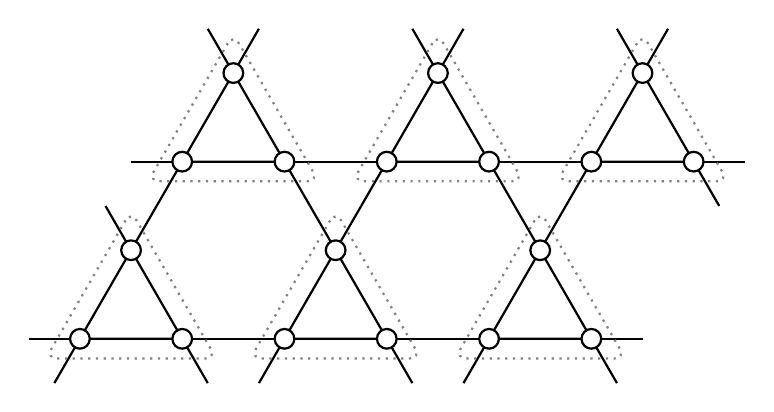
\begin{tikzpicture}

        \def\disT{0.750}
        \def\tensorSize{0.125}

        % \begin{scope}[shift = {(-4.5, +3.25)}]
        %     \draw[thick, -{Stealth[scale = 1.0]}] (0 : 0) to (240 : 1.0) node at (240 : 1.25) {$x$};
        %     \draw[thick, -{Stealth[scale = 1.0]}] (0 : 0) to (  0 : 1.0) node at (  0 : 1.25) {$y$};
        % \end{scope}

        \foreach \x in {-6, -2, +2} {

            \foreach \y in {0} {

            \begin{scope}[shift = {({\x*\disT*cos(30)}, \y*\disT)}]

                    \coordinate (T1) at (210 : \disT);
                    \coordinate (T2) at ( 90 : \disT);
                    \coordinate (T3) at (330 : \disT);

                    % draw inter-layer T1-T2-T3
                    \draw[thick] (T1) to (T2) to (T3) -- cycle;
                    \draw[thick] (T1) to ($(T1) + (180 : {1.0 * cos(30) * \disT})$);
                    \draw[thick] (T1) to ($(T1) + (240 : {1.0 * cos(30) * \disT})$);
                    \draw[thick] (T2) to ($(T2) + ( 60 : {1.0 * cos(30) * \disT})$);
                    \draw[thick] (T2) to ($(T2) + (120 : {1.0 * cos(30) * \disT})$);
                    \draw[thick] (T3) to ($(T3) + (  0 : {1.0 * cos(30) * \disT})$);
                    \draw[thick] (T3) to ($(T3) + (300 : {1.0 * cos(30) * \disT})$);

                    \foreach \T in {T1, T2, T3} {
                        \draw[thick, fill = white] (\T) circle (\tensorSize);
                    }

                    % draw unit cell borders
                    \draw[thick, gray, dotted, rounded corners] ($(T2) + (90 : 0.50)$) to ($(T1) + (210 : 0.50)$) to ($(T3) + (330 : 0.50)$) -- cycle;

                \end{scope}

            }

        }

        \foreach \x in {-4, 0, +4} {

            \foreach \y in {+4.0} {

                \begin{scope}[shift = {({\x*\disT*cos(30)}, {\y*\disT*cos(30)*tan(60)/2})}]

                    \coordinate (T1) at (210 : \disT);
                    \coordinate (T2) at ( 90 : \disT);
                    \coordinate (T3) at (330 : \disT);

                    % draw inter-layer T1-T2-T3
                    \draw[thick] (T1) to (T2) to (T3) -- cycle;
                    \draw[thick] (T1) to ($(T1) + (180 : {1.0 * cos(30) * \disT})$);
                    \draw[thick] (T1) to ($(T1) + (240 : {1.0 * cos(30) * \disT})$);
                    \draw[thick] (T2) to ($(T2) + ( 60 : {1.0 * cos(30) * \disT})$);
                    \draw[thick] (T2) to ($(T2) + (120 : {1.0 * cos(30) * \disT})$);
                    \draw[thick] (T3) to ($(T3) + (  0 : {1.0 * cos(30) * \disT})$);
                    \draw[thick] (T3) to ($(T3) + (300 : {1.0 * cos(30) * \disT})$);

                    \foreach \T in {T1, T2, T3} {
                        \draw[thick, fill = white] (\T) circle (\tensorSize);
                    }

                    % draw unit cell borders
                    \draw[thick, gray, dotted, rounded corners] ($(T2) + (90 : 0.50)$) to ($(T1) + (210 : 0.50)$) to ($(T3) + (330 : 0.50)$) -- cycle;

                \end{scope}

            }

        }

    \end{tikzpicture}

\end{document}

%%% Local Variables:
%%% mode: latex
%%% TeX-master: t
%%% End:
